\documentclass[11pt]{article}
\usepackage[a4paper,top=3cm,bottom=3cm,left=2.5cm,right=2.5cm]{geometry}
\usepackage[italian]{babel}
\usepackage[utf8x]{inputenc}
\usepackage {caption}
\usepackage {url}
\usepackage {multirow}
\usepackage {booktabs}
\usepackage {fixltx2e}
\usepackage {float}
\usepackage {graphicx}
\usepackage {cite}
\usepackage {listings}
\usepackage {color}
\usepackage {xcolor,colortbl}
\usepackage {adjustbox}
\usepackage {array}
\usepackage {svg}
\usepackage {subfig}
\usepackage {amssymb}
\usepackage {hyperref}
\usepackage {tabulary}
\usepackage {tabularx}
\usepackage[T1]{fontenc}
\usepackage{wasysym}
\usepackage{enumitem}

\newcommand{\voceU}[1]{%
	\item #1\dotfill\Square%
}

\newcommand{\voceD}[1]{%
	\item #1\hfill\Square%
}
\hypersetup{colorlinks=true,citecolor=black,linkcolor=black, urlcolor=blue}

\date{}

\renewcommand{\lstlistingname}{Listato}


\lstset{
    language=C,
    basicstyle=\ttfamily,
    breaklines=true,
    frame=single, % draw a frame at the top and bottom of the code block
    tabsize=2, % tab space width
    showstringspaces=false, % don't mark spaces in strings
    numbers=left, % display line numbers on the left
    captionpos=b,
    commentstyle=\color{green}, % comment color
    keywordstyle=\color{blue}, % keyword color
    stringstyle=\color{red} % string color
}

\begin{document}

\title{\textbf{Definizione ed Implementazione di un Sistema di Raccomandazione Distribuito per film
		e Modellazione di Eventi Complessi}}

\author{\\\textit{Prof.} Ing. Tommaso di Noia\\\textit{Prof.ssa} Marina Mongiello \\
	Mauro Losciale\\ 
	Pietro Tedeschi\\}

\clearpage\maketitle
\thispagestyle{empty}

\begin{center}
	
\includegraphics[scale=0.40]{images/poliba.jpg}
\end{center}

{\textbf{\center Logica e Intelligenza Artificiale\\Ingegneria del Software Avanzata\\ Laurea Magistrale in Ingegneria Informatica\\Politecnico di Bari\\A.A 2015 - 2016\\}}

\newpage
\clearpage
\thispagestyle{empty}
\renewcommand\contentsname{Indice}
\tableofcontents
\newpage
\setcounter{page}{1}
\section{Introduzione al progetto}
''\emph{The Grid is a software infrastructure that enables flexible, secure, coordinated resource sharing among dynamic collections of individuals, institutions and resources.}'' (Foster e Kesselman, 1998).

Lo sviluppo ed il progresso tecnologico avutosi attraverso la scienza e l'ingegneria, richiede ogni giorno un incremento della \emph{potenza computazionale}. Il Grid Computing oltre ad essere in grado di rispondere a tale necessità, fornisce un aumento della \emph{capacità di storage} per il calcolo scientifico.
Quando si parla di scienza, ci si sta riferendo in linea generale a tutte quelle discipline come la fisica, la chimica, l'ingegneria, la medicina e così via, le quali raccolgono quotidianamente un ammontare di dati, organizzati e strutturati all'interno di database \cite{2} \cite{3}.

L'obiettivo del progetto è analizzare come i database possano essere integrati all'interno di griglie computazionali, in modo da far si che le molteplici applicazioni possano accedere di conseguenza ai dati, memorizzati all'interno di una struttura. Ciò non risulta possibile adottando semplicemente i noti componenti per la gestione dei file nell'ambito del \textbf{Grid Computing}, poiché bisogna tener conto delle transazioni, e quindi delle query effettuate sulla base di dati. Un aspetto rilevante inoltre, è quello della \textbf{eterogeneità} tra i differenti \textbf{DataBase Management System} (DBMS). Oltre alle note differenze tra il paradigma ad oggetti, quello relazionale, ed i database \emph{eXtensible Markup Language} (XML), i prodotti come ad esempio \emph{Oracle} e \emph{DB2} differiscono sia nelle funzionalità che nelle interfacce. Questa diversità, crea una notevole complessità nella progettazione di una particolare soluzione per l'integrazione dei database all'interno di una griglia computazionale, poichè i dati devono essere combinati tra di loro. Tuttavia questo sforzo viene compensato da una migliore produttività ed un'efficiente interazione tra i differenti paradigmi \cite{2} \cite{3}.

Uno degli obiettivi del Grid Computing, consiste proprio nell'incentivare lo sviluppo ed il progresso scientifico secondo una filosofia più incentrata sul concetto di Open. Si pensi ai vantaggi che si possono ottenere combinando dati provenienti da sorgenti differenti, al fine di produrre nuovi risultati.
Pertanto, è importante disporre di un front end (\textbf{middleware}) a supporto del Grid Computing al fine di interconnettere le differenti basi di dati.

In sintesi, gli obiettivi prefissati sono:
\begin{enumerate}
\item Fornire un accesso autorizzato e sicuro ai database distribuiti sulla rete Internet, mediante l'utilizzo del \emph{Grid Security Infrastructure} (GSI), con il supporto  ai certificati \emph{X.509}.
\item Un metodo di accesso comune ed una gestione delle transazioni su database distribuiti per i differenti paradigmi dei database.
\item Incremento dell'efficienza computazionale,produttività ed interoperabilità.
\end{enumerate}
\section{Database Eterogenei Distribuiti}

In questa sezione saranno evidenziati i punti cardine per l'implementazione di un database distribuito eterogeneo in una Griglia Computazionale.

Una delle caratteristiche principali di una Griglia Computazionale è \emph{l'eterogeneità}, ovvero l'essere costituita da risorse differenti con caratteristiche diverse, mostrate all'utente finale come parte di un unico sistema. Ad esempio, in una griglia è possibile avere due cluster aventi processori con architetture diverse o software diversi, oppure nello stesso cluster è possibile avere macchine con risorse differenti.

Questa proprietà è valida nell'ambito dei \emph{DBMS}. Abbiamo diverse tipologie di basi di dati utilizzate nelle applicazioni informatiche: relazionali, XML, CSV o semplicemente un file di testo. Tuttavia, gli utenti della Griglia accedono a tali dati senza distinguere la struttura fisica nella quale sono organizzati, o l'effettiva locazione geografica.

Il riferimento principale nello sviluppo di database distribuiti su Griglie è dato dall'architettura orientata ai servizi \textbf{OGSA (Open Grid Service Architecture)}. L'architettura OGSA semplifica notevolmente lo sviluppo di sistemi Grid-based sicuri e robusti, ed offre agli sviluppatori la possibilità di implementarne i componenti garantendo interoperabilità, riusabilità e portabilità degli stessi. L'idea dei Grid Service è quella di estendere le funzionalità web cosiddette \emph{well-defined}, definite dagli standard (WSDL, XML Schema, SOAP, etc.) per il supporto alle caratteristiche delle Grid \cite{2} \cite{3}. 

In Figura \ref{accessogrid} è riportato lo schema logico del \emph{message flow} tra i client e i dati nelle Grid, proposto dal Global Grid Forum nel Grid Database Service Specification. Ciò consente di accedere ai dati e modificarne il contenuto o la struttura. 

Il \textbf{Grid Data Service (GDS)} è un tipo di \emph{wrapper} accessibile dall'esterno. I client scambiano i dati con i DBMS attraverso un GDS, il quale funziona a livello logico come "proxy". Inoltre, i GDS devono necessariamente supportare i comuni standard utilizzati nei DBMS, ad esempio SQL, prevedendo meccanismi di autenticazione per l'accesso alle risorse, conformi alle specifiche sulle Grid. Il \textbf{Grid Data Service Factory} è il componente utilizzato per generare i GDS (al contrario dei \emph{Web Service}, dove una Factory non è necessaria) \cite{3}. 

\begin{figure}[H]
\centering
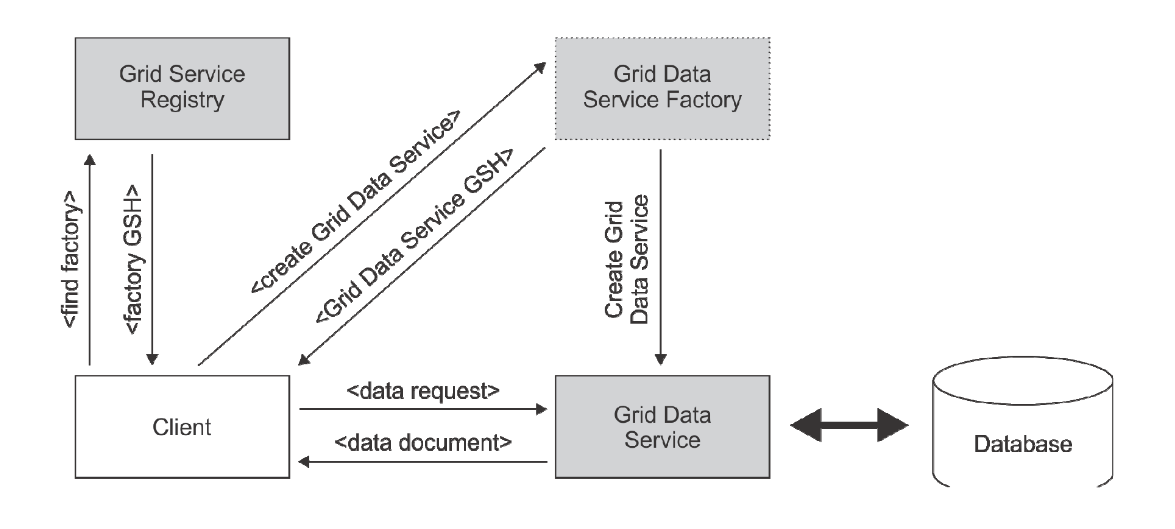
\includegraphics[scale=0.40]{images/agds.png}
\caption{Accesso e modifica di un dato in una Grid utilizzando un Grid Data Service \cite{2}}
\label{accessogrid}
\end{figure}


In Figura \ref{archgridatabase} viene presentata una possibile architettura di un \emph{Grid Database System}, tenendo presente quanto descritto precedentemente riguardo le differenti tipologie di risorse e la loro dislocazione. In accordo con quanto descritto, è necessaria l'installazione di un DBMS in ogni nodo della Grid. 

\begin{figure}[H]
\centering
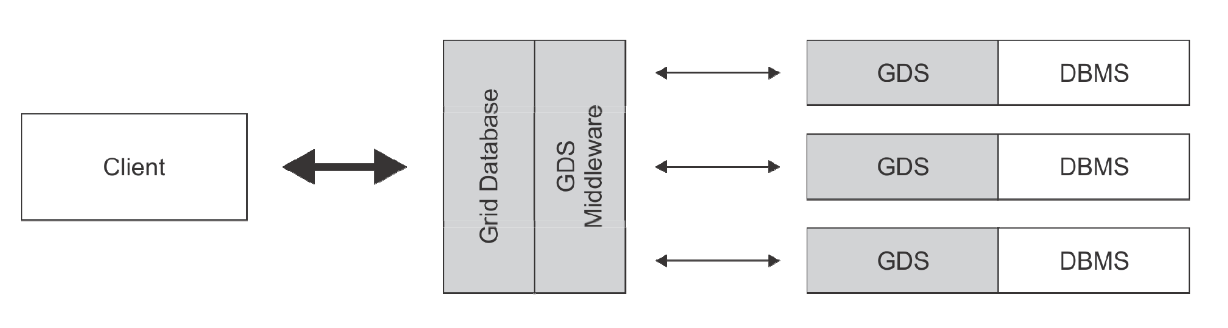
\includegraphics[scale=0.40]{images/archgrid.png}
\caption{Architettura di un Grid Database System \cite{2}}
\label{archgridatabase}
\end{figure}

Considerando che i DMBS attuali sono sistemi sviluppati, utilizzati e testati da molti anni in maniera rigorosa, si è scelto di utilizzare tali tecnologie già presenti all'interno delle infrastrutture. Per interconnettere le diverse tecnologie, il lavoro principale da svolgere è l'implementazione dei GDS, ad esempio come parte di un \textbf{Grid Data Service Middleware}. Esso è un altro tipo di wrapper per sistemi Grid Database complessi, che garantisce la cosiddetta \emph{trasparenza}. Per trasparenza si intende una serie di proprietà, quali locazione, nome del database, distribuzione e replica dei dati, eterogeneità, proprietà e costi. 

Infine è utile citare altri possibili modi per implementare un Grid Database System. Si potrebbe pensare, ad esempio, di immagazzinare i dati nella memoria centrale, oppure utilizzare una struttura client-server centralizzata, o servizi basati su \emph{Remote Procedure Call}. Queste tipologie di organizzazione dei dati, tuttavia, riscontrano molti problemi quando le applicazioni fanno uso di un'enorme quantità di dati, tuttavia non sfruttando a pieno le potenzialità computazionali di una Grid \cite{3}.

\newpage

\subsection{Questionario di Autovalutazione}

\textbf{Descrivere il concetto di eterogeneità in una griglia computazionale.}\\[4ex]
\rule[5mm]{\textwidth}{0.1mm} 
\rule[5mm]{\textwidth}{0.1mm}
\rule[5mm]{\textwidth}{0.1mm} 
\textbf{Descrivere brevemente i componenti dell'architettura OGSA ed il loro funzionamento.}\\[4ex]
\rule[5mm]{\textwidth}{0.1mm} 
\rule[5mm]{\textwidth}{0.1mm}
\rule[5mm]{\textwidth}{0.1mm} 
\rule[5mm]{\textwidth}{0.1mm}
\rule[5mm]{\textwidth}{0.1mm} 
\textbf{Un Grid Data Service Middleware garantisce la proprietà di}
\begin{enumerate}
	\voceU{Interoperabilità}
	\voceU{Trasparenza}
	\voceU{Scalabilità}\\
\end{enumerate}
\textbf{Disegnare lo schema architetturale di un Grid Database System.}\\\\\\\\\\\\\\\\\\\\\\\\\\\\\\\\\\
\textbf{Quale fattore tra i seguenti incide negativamente su di un Grid Database System implementato tramite architetture classiche (RPC, Client-Server)?}
\begin{enumerate}
	\voceU{Implementazione complessa}
	\voceU{Enorme quantità di dati}
	\voceU{Numero di nodi nella griglia}\\
\end{enumerate}
\newpage

\section{Stato dell'Arte}
In questa sezione illustriamo alcune delle architetture sviluppate per l'integrazione di database eterogenei attraverso le Grid. Tra i progetti presi in considerazione abbiamo \textbf{GISE}, \textbf{OGSA-DQP} e \textbf{GDIS}, illustrati di seguito. \\

\textbf{GISE (Grid Integration SErvice)} è un'architettura per l'accesso e l'integrazione di basi di dati sviluppata sull'infrastruttura Grid offerta da \textbf{\emph{Globus Toolkit 4}}. Originariamente progettata per il monitoraggio delle epidemie, utilizza un sistema basato sul \emph{Canonical Data Model} per l'esecuzione di query su database geograficamente distribuiti. Un layer chiamato \emph{Mediator} raccoglie le richieste per l'accesso ai dati integrati, convertendo le query a seconda della tecnologia del RDBMS sottostante. Questa tecnica è vantaggiosa dal punto di vista della scalabilità del sistema ma può creare \emph{bottleneck} a livello centrale del sistema \cite{archgrid}. \\

\textbf{OGSA-DQP} (Distributed Query Processing) è un componente di OGSA-DAI (Open Grid Services Architecture Data Access and Integration) che mette a disposizione un servizio in grado di effettuare query multiple in differenti database, tramite una sola richiesta (query) iniziale. DQP partiziona la query in sottoquery, ognuna delle quali è effettuata sul DB opportuno. Al fine di integrare le diverse tipologie di dati provenienti dai database distribuiti, utilizza tecniche di parallelizzazione ed unione dei dati. E' necessario, tuttavia, memorizzare in primis gli schemi relativi ai DBMS da interrogare: per fare ciò gli sviluppatori hanno a disposizione la funzione \emph{ImportSchema}. Questa operazione configura automaticamente anche il modulo GDQS (Grid Distributed Query Service), il quale abilita l'accesso ai dati geograficamente distribuiti. L'integrazione effettuata da OGSA-DQP è di tipo verticale, ovvero estrae ed unisce i dati per colonne, creando una vista sulla quale effettuare la query \cite{archgrid}.\\

\textbf{GDIS} (Grid Data Integration Service) propone di estendere le funzionalità di OGSA-DQP tramite un approccio decentralizzato, basato su reti Peer-to-Peer (P2P) \cite{comito2004gdis}.

\subsection{Architettura per l'integrazione}

In questa sezione illustriamo l'architettura di base per l'integrazione di database eterogenei distribuiti. Lo scenario comune prevede l'interconnessione di RDBMS forniti da diversi vendors e localizzati in diversi domini amministrativi, creando una singola "vista" del sistema, unica e trasparente all'utente. Tuttavia, l'integrazione non deve alterare la struttura dei singoli sistemi a livello locale, in termini di condivisione e policies dei dati.

Attraverso il tool OGSA-DAI è possibile "esporre" le diverse tecnologie come risorsa della Grid, avendo a disposizione un'interfaccia standard per l'accesso. In Figura \ref*{propintegr} sono mostrati differenti approcci per l'integrazione, sia nel caso in cui i DB sono presenti nello stesso dominio amministrativo e nel caso di domini e hosting differenti \cite{archgrid}.

\begin{figure}[H]
\centering
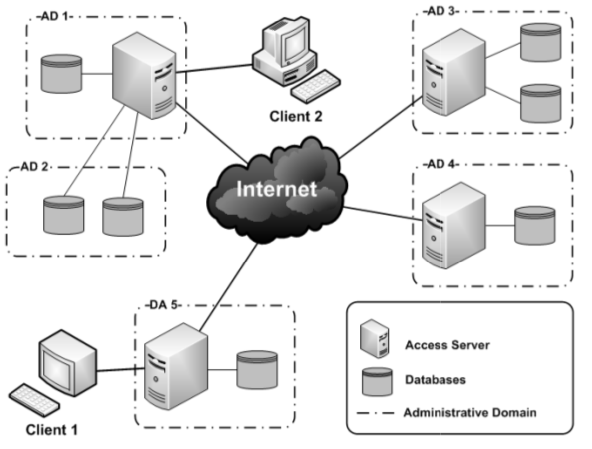
\includegraphics[scale=0.50]{images/datainteg.png}
\caption{Proposte di Data Integration \cite{archgrid}}
\label{propintegr}
\end{figure}

Tra le varie configurazioni è presente un Access Server (AC) a ridosso di uno o più database dello stesso dominio, al fine di amministrare gli accessi alle risorse. Un Access Server può accedere in maniera diretta al DB oppure delegare l'accesso ad un altro AC. Questo tipo di integrazione facilita la scalabilità del sistema, prevedendo la sola aggiunta/rimozione di una risorsa della Grid nel caso di modifiche ai database, in modo completamente trasparente all'utente. In Figura \ref{imple} è mostrato lo schema implementativo proposto \cite{archgrid}. 

\begin{figure}[H]
	\centering
	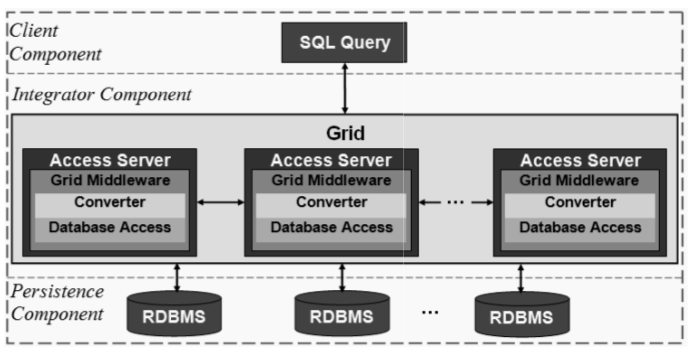
\includegraphics[scale=0.50]{images/schemaimpl.png}
	\caption{Implementazione }
	\label{imple}
\end{figure}

\subsection{DIGE Framework}

I componenti utilizzati per l'integrazione e la condivisione dei dati sono mostrati in Figura \ref{dige}, e l'architettura composta da tali elementi è chiamata \textbf{DIGE} (Database Integration using Grid Environment). I 3 elementi principali di DIGE sono : 
\begin{itemize}
\item Il \textit{Client Component}, basato su OGSA-DAI Client Toolkit, utilizzato da DIGE per l'esecuzione dei comandi nella Grid. I client, attraverso tale strumento, possono eseguire dei task chiamati \textit{Activities}, organizzati secondo un \textit{Workflow} il quale viene processato in sequenza dall'Access Server. Tale struttura offre una serie di vantaggi anche dal punto di vista dello sviluppo: il layer, infatti, nasconde la complessa struttura di OGSA-DAI, mettendo a disposizione API semplici per implementare i meccanismi di invio/ricezione dei risultati negli applicativi Grid. E' garantita inoltre piena compatibilità delle applicazioni grazie all'integrazione dei \textbf{Driver JDBC}, sviluppati in Java \cite{archgrid}.
\item L'\textit{Integrator Component}, basato su Globus Toolkit 4 (GT4) e OGSA-DQP, utilizza le funzionalità di \textbf{QCONG-G}. Esso riceve il Worflow generato dal client e coordina la sua esecuzione. Il modulo GT4 è responsabile della sicurezza e l'accesso alle risorse richieste dai processi. Effettua un forwarding del Worflow, tramite una richiesta HTTP nel quale è incapsulato un messaggio SOAP, al modulo OGSA-DAI, il quale localizza i database ed esegue i task opportuni. 
\item Il \textit{Persistence Component}, il quale si occupa dell'integrità dei dati e della rappresentazione verso le varie tecnologie RDBMS supportate da OGSA-DAI, inclusi PostgreSQL, MySQL, Oracle e IBM DB2 \cite{archgrid}.
\end{itemize}	

\begin{figure}[H]
	\centering
	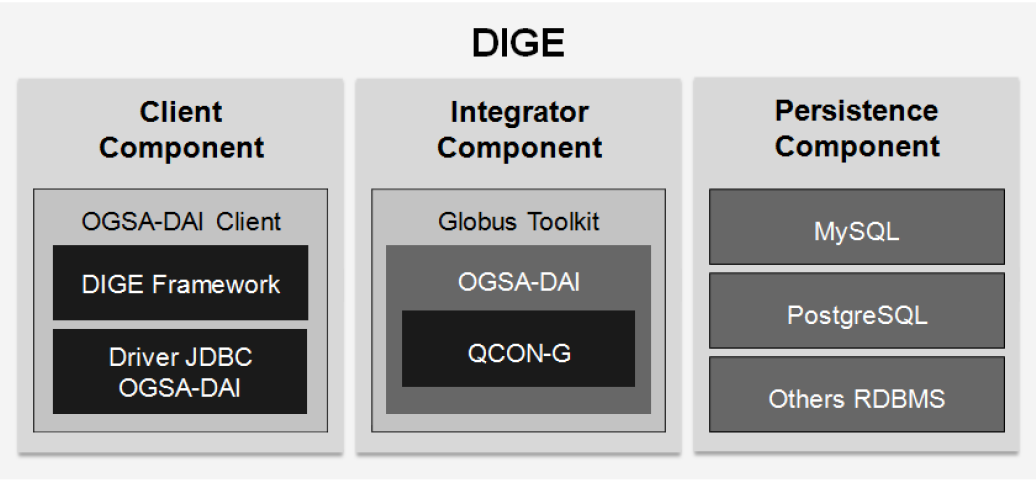
\includegraphics[scale=0.50]{images/dige.png}
	\caption{Architettura DIGE \cite{archgrid}}
	\label{dige}
\end{figure}

\subsubsection{QCON-G}
Il modulo QCON-G ricopre un ruolo fondamentale nel flusso di esecuzione di DIGE, ovvero è responsabile dell'accesso ai diversi schemi logici relazionali presenti, al fine di creare un'unica vista per l'utente finale \cite{archgrid}. 

\begin{figure}[H]
	\centering
	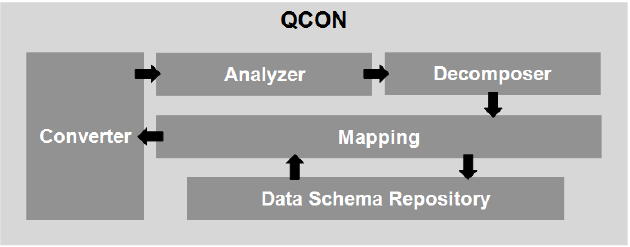
\includegraphics[scale=0.50]{images/qcon.png}
	\caption{Modulo QCON \cite{archgrid}}
	\label{qcon}
\end{figure}

Tra le funzionalità di QCON abbiamo: 
\begin{itemize}
	\item \textit{Converter}: E' il meccanismo che coordina l'intero modulo QCON. Riceve le query e le invia al componente Analyzer, ed al termine del processo genera una nuova query in base alle informazioni ricevute dal Mapping Module.
	\item \textit{Analyzer}: Si occupa principalmente dell'analisi lessicale e sintattica delle query.
	\item \textit{Decomposer}: Dopo l'analisi la query viene suddivida dal modulo Decomposer in simboli ed unità atomiche del linguaggio SQL, come nomi di tabelle e colonne, costanti, operatori etc.
	\item \textit{Mapping}: Attraverso la lista delle unità atomiche fornita dal Decomposer, il modulo Mapping associa a tali informazioni i corrispondenti schemi relazionali, forniti dal Data Schema Repository, restituendo tale lista al modulo Converter \cite{archgrid}.
\end{itemize}

\subsection{FirstDIG}

Il progetto \textbf{FirstDIG} (First Data Investigation on the Grid) nasce nel 2004 dalla collaborazione tra Firstgroup PLC, una delle società di trasporti leader nel settore in Regno Unito, ed il centro di ricerca nazionale (NesC). Esso propone, attraverso una recente implementazione di OGSA-DAI, un sistema Grid a livello commerciale, in grado di estrarre informazioni dalla rilevazione del numero di ticket giornalieri, arrivi e partenze dei bus, contatti con i clienti e chilometraggio dei veicoli, attraverso un processo di Data Mining. Al seguente link è possibile consultare la pagina ufficiale del progetto ed il suo stato attuale: \url{http://www.epcc.ed.ac.uk/firstdig/} \cite{Sloan_firstdata}

\subsection{ADMIRE - Advanced Data Mining and Integration Research for Europe}

\textbf{ADMIRE} è l'acronimo di \emph{Advanced Data Mining and Integration Research for Europe}. Il progetto, della durata di 3 anni, viene coordinato dall'Università di Edinburgo, con la collaborazione delle seguenti università e realtà aziendali: University of Vienna, Universidad Politécnica de Madrid, Ústav informatiky, Slovenská akadémia vied, Fujitsu Labs of Europe, ComArch S.A. \cite{6020018}.

ADMIRE ha lo scopo di sviluppare un'architettura dati orientata ai servizi, flessibile, nel campo della distribuzione ed integrazione dei dati su larga scala. L'obiettivo è quello di introdurre nuove funzionalità al fine di integrare informazioni da risorse eterogenee, ed aiutare i ricercatori e gli analisti, sia a chiedere che a rispondere alle nuove domande nel campo scientifico ed in quello della Business Intelligence \cite{6020018}.

Oggi si assiste all'incremento esponenziale relativo alla crescita dei dati. Tecnologie avanzate di memorizzazione, sistemi pervasivi, sensori digitali e reti di comunicazione che collezionano elevate e complesse quantità di informazioni di massa all'interno dei \textbf{Data Repository}. Tipicamente, per consentire l'estrazione della conoscenza da molteplici risorse eterogenee distribuite, sono necessarie tecniche di data mining. Oggi, gli ingegneri, manutentori, responsabili delle decisioni o i ricercatori, hanno notevoli difficoltà nell'estrarre le informazioni. Quindi al fine di poter recuperare informazioni da diverse sorgenti distribuite, è utile conoscere in dettaglio, la sorgente dei dati, il meccanismo per l'integrazione, e le strategie di data mining \cite{6020018}.

ADMIRE è un progetto che consente di incrementare la velocità nell'accesso alle informazioni, e di ricavare benefici inerenti alla valorizzazione dei dati da parte dell'economia e della comunità Europea. Ciò avviene con estrema facilità nascondendo tutti i dettagli realizzativi e le tecnologie usate all'utente finale, fornendo a quest'ultimo una semplice interfaccia \cite{6020018}.

All'interno del progetto ADMIRE vengono esaminati nel dettaglio due scenari per testare la propria tecnologia, nei seguenti ambiti:
\begin{enumerate}
	\item \textbf{Flood modelling and simulation}
	\item \textbf{Customer Relationship Management}
\end{enumerate}
Il \emph{Flood modelling and simulation} è un insieme di modelli meteorologici, idrologici ed idraulici, che insieme consentono agli utenti di predire disastri alluvionali, utilizzando le previsioni meteorologiche.

Il \emph{Customer Relationship Management} fornisce il supporto per il "front office" business, includendo le vendite, il marketing ed i servizi.

L'infrastruttura di ADMIRE, sarà in grado di comunicare con una serie di gateway tra loro connessi mediante Internet e la rete Grid. La comunicazione avviene utilizzando uno standard sviluppato da ADMIRE sull'\emph{Infrastructure Service Bus} (ISB). Ogni gateway fornisce un insieme di servizi per l'integrazione, usabili mediante un linguaggio ed un'architettura ad alto livello \cite{6020018}.

\begin{figure}[H]
	\centering
	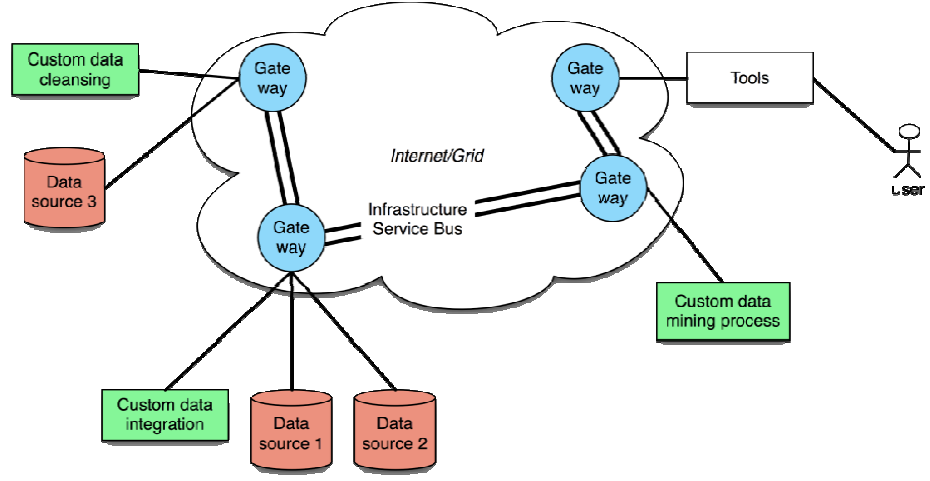
\includegraphics[scale=0.65]{images/admirearch.png}
	\caption{Architettura di ADMIRE \cite{6020018}}
	\label{admirearch}
\end{figure}

\newpage

\subsection{Questionario di Autovalutazione}
\textbf{Descrivere i componenti ed il funzionamento del modulo QCON-G.}\\[5ex]
\rule[5mm]{\textwidth}{0.1mm} 
\rule[5mm]{\textwidth}{0.1mm} 
\rule[5mm]{\textwidth}{0.1mm} 
\rule[5mm]{\textwidth}{0.1mm} 
\rule[5mm]{\textwidth}{0.1mm} 
\textbf{La comunicazione tra i gateway nell'architettura di ADMIRE, avviene su: }
\begin{enumerate}
	\voceU{Infrastructure Service Bus (ISB)}
	\voceU{Front Side Bus (FSB)}
	\voceU{Process Field Bus (PFB)}\\
\end{enumerate}
\textbf{In DIGE i componenti principali sono:}
\begin{enumerate}
	\voceU{Client Component, Server Component, Persistence Component}
	\voceU{ Client Component, Integrator Component, Persistence Component}
	\voceU{Client Component, Data Component, Map Component}\\
\end{enumerate}
\textbf{Descrivere cosa sono Flood modelling and simulation e Customer Relationship Management.}\\[5ex]
\rule[5mm]{\textwidth}{0.1mm} 
\rule[5mm]{\textwidth}{0.1mm} 
\rule[5mm]{\textwidth}{0.1mm} 
\rule[5mm]{\textwidth}{0.1mm} 
\rule[5mm]{\textwidth}{0.1mm} 
\textbf{Disegnare lo schema implementativo proposto per il Data Integration.}
\newpage


\section{Esempio pratico - OGSA-DAI WSRF}
\subsection{Web Service Resource Framework}
Le interfacce dei servizi Web spesso hanno la necessità di fornire delle interazioni con stato con i relativi client del servizio (ad esempio, un'interfaccia del servizio Web come un carrello della spesa, dove il risultato di un'operazione, influenza l'esecuzione delle operazioni successive). \textbf{WSRF} (\emph{Web Services Resource Framework}) di \textbf{OASIS} definisce un generico framework per la creazione e l'accesso alle risorse con stato mediante l'utilizzo dei servizi Web, in modo che la definizione, l'implementazione, l'integrazione e la gestione del servizio stesso, risultino più semplici \cite{ogsadai}.\\

WSRF introduce il concetto di descrizione di un documento XML, denominato schema del documento delle proprietà delle risorse, al quale fa riferimento la descrizione \textbf{WSDL} di un servizio web. Lo schema inoltre, descrive esplicitamente una vista dello stato della risorsa con la quale il client interagisce. Un servizio così descritto viene chiamato \textbf{WS-Resource} \cite{ogsadai}.\\

Una \emph{WS-Resource}, viene definita come la combinazione di una risorsa e di un servizio Web tramite cui si accede alla risorsa stessa. La Figura \ref{wsrf} illustra un servizio Web, definito su\\ \emph{http://www.example.com/service}, e tre risorse, \textbf{A}, \textbf{B} e \textbf{C}. Nella Figura \ref{wsrf} vengono illustrate tre WS-Resources:

\begin{figure}[H]
	\centering
	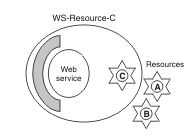
\includegraphics{images/wsresource.png}
	\caption{WS Resource}
	\label{wsrf}
\end{figure}

Si indica una WS-Resource mediante il riferimento ad un end-point di \textbf{WS-Addressing} che identifica univocamente la WS-Resource, solitamente contenente un identificativo del componente della risorsa della WS-Resource, all'interno dell'elemento \emph{EndpointReference ReferenceParameter}. Nell'esempio precedente, \emph{WS-Resource-C} è la combinazione del servizio Web e della risorsa identificata da \emph{C}. Un esempio del riferimento a WS-Resource-C che potrebbe comparire è il seguente:
\\
\lstset{
	language=XML,
	numbers=none,
	morekeywords={encoding,
		xs:schema,xs:element,xs:complexType,xs:sequence,xs:attribute}
}
\lstset{
	language        = bash,
	basicstyle      = \small\ttfamily,
	breaklines      = true,
	numbers=none,
	keywordstyle    = \color{blue},
	stringstyle     = \color{red},
	identifierstyle = \color{black},
	commentstyle    = \color{orange},
	emph            =[1]{php},
	emphstyle       =[1]\color{black},
	showstringspaces=false,
	emph            =[2]{if,and,or,else},
	emphstyle       =[2]\color{yellow}}

\begin{lstlisting}
<wsa:EndpointReference>
<wsa:Address>
http://www.example.com/service
</wsa:Address>
<wsa:ReferenceParameters>
<tns:SomeDisambiguatorElement>C</tns:SomeDisambiguatorElement>
</wsa:ReferenceParameters>
...
</wsa:EndpointReference>
\end{lstlisting}

Ciascuna di queste WS-Resource ha un documento che definisce le proprietà della risorsa (un documento dell'istanza XML), il quale descrive una vista dello stato della risorsa. Il \emph{WSDL} per una WS-Resource identifica lo schema XML che descrive la tipologia di documento delle proprietà delle risorse tramite un attributo \emph{ResourceProperties} dell'elemento \emph{wsdl:PortType}. Specificando questa estensione standard di WSDL inerente allo schema del documento delle proprietà della risorsa, WSRF consente la definizione di semplici messaggi generici che interagiscono con la WS-Resource \cite{ogsadai}.

\subsection {Perform Document}
I \textbf{Perform Document} vengono utilizzati dai client al fine di consentire ad un servizio dati l'esecuzione di determinate attività. Queste attività comprendono l'utilizzo di risorse dati, l'esecuzione di query, aggiornamenti, conversioni relative al formato dati ed operazioni di trasmissione/ricezione \cite{ogsadai}. 

Ad esempio, un perform document potrebbe specificare la costruzione di una singola query su un database, oppure nel caso più complesso, l'interconnessione di diverse attività, contenute all'interno di una pipeline. Inoltre, anche il risultato di una query su un database, potrebbe essere filtrato, trasformato e successivamente inviato mediante il protocollo FTP all'interno di una pipeline di attività \cite{ogsadai}.

Il vantaggio di sfruttare la tecnica della pipeline, consente di eliminare lo spostamento superfluo dei dati. Ciò si ottiene spostando la computazione, direttamente sul dato sorgente, consentendo al dato stesso di essere elaborato dalle molteplici attività. Se ogni attività che viene istanziata, utilizza un proprio servizio, oppure effettua una propria richiesta, si potrebbe incorrere in un \emph{overhead} provocato dalla serializzazione, de-serializzazione e trasporto dei dati in rete \cite{ogsadai}.

I perform document vengono utilizzati anche per la specifica dei requisiti di sessione relativi ad una richiesta. Ad esempio, un perform document, può richiedere ad un servizio dati, di creare una nuova sessione dotata di una durata limitata. Le attività descritte con un perform document consentono di accedere ad una sessione al fine di memorizzarne lo stato, il quale sarà reso disponibile mediante una semplice richiesta alla sessione stessa \cite{ogsadai}.

Le \textbf{Client Toolkit API} fornite con \textbf{OGSA-DAI}, danno la possibilità agli sviluppatori Java, di costruire applicazioni che generano perform document e di interpretarne i risultati.

\begin{figure}[H]
	\centering
	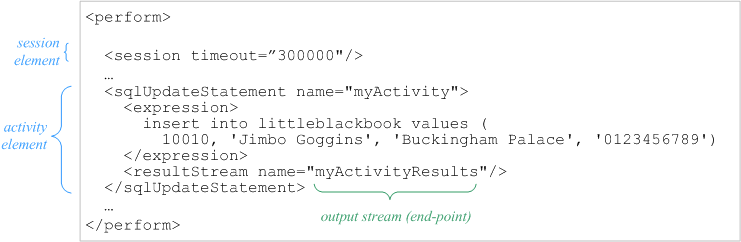
\includegraphics[scale=0.60]{images/PerformDocument.png}
	\caption{Un semplice perform document contenente un elemento session, activity ed end-point.}
	\label{admirearch}
\end{figure}

I perform document vengono definiti mediante il linguaggio \emph{XML}. La radice di un perform document, è un elemento \textbf{$<$perform$>$}, dove sotto il quale può trovarsi un altro elemento opzionale denominato \textbf{$<$session$>$} con una o più attività. L'elemento \textbf{$<$session$>$} viene utilizzato per specificare i requisiti di sessione relativi alla richiesta effettuata. Un elemento attività, è un elemento che rappresenta un funzione per una determinata risorsa relativa ad un servizio dati \cite{ogsadai}. 

Tutti gli elementi attività contenuti all'interno di un perform document devono possedere l'attributo nome, definito in maniera univoca. Le attività possono essere connesse al fine di costituire una pipeline, assicurandosi che  l'output di un elemento attività sia l'input per un altro. Qualsiasi output non connesso, prende il nome di \textbf{end-point} di perform document. I dati contenuti all'interno di questi end-point saranno inviati al client con un documento di riscontro \cite{ogsadai}.

\subsection{Installazione di OGSA-DAI WSRF}

L'installazione del framework è stata effettuata su ambiente Unix, in particolare utilizzando la distribuzione \textbf{Ubuntu 12.04}. Prima di procedere, sono necessari dei tool preliminari per la configurazione e l'esecuzione del framework: 
\begin{itemize}
	\item \textbf{Java 1.4.x} o superiore.
	\item \textbf{Apache ANT} \url{http://ant.apache.org}.
	\item \textbf{Globus Toolkit 4.0.2 Java Web Services Core}, implementazione base di WSRF in Java, utilizzata da OGSA-DAI come \emph{Web Container} \cite{ogsadai}.
\end{itemize}

Scarichiamo i binari dal repository ufficiale \url{http://sourceforge.net/projects/ogsa-dai/files/archive/ogsadai2.2/ogsadai-wsrf-2.2-bin.tar.gz/download} e configuriamo le variabili d'ambiente per referenziare correttamente il core: 


\begin{lstlisting}[language=bash]
$ export GLOBUS_LOCATION=/path/to/Globus/directory
\end{lstlisting}
Spostiamoci nella directory principale ed eseguiamo il seguente comando per l'installazione tramite \textbf{GUI}: 
\begin{lstlisting}[language=bash]
$ ant guiInstall
\end{lstlisting}

Seguiamo i vari step indicati nella guida, ed una volta completata la procedura clicchiamo su \textbf{Finish}.

\subsection{Creazione di un Data Service}

Nella directory di OGSA-DAI WSRF lanciamo il seguente comando: 

\begin{lstlisting}[language=bash]
$ ant guiDeployService
\end{lstlisting}

\begin{figure}[H]
	\centering
	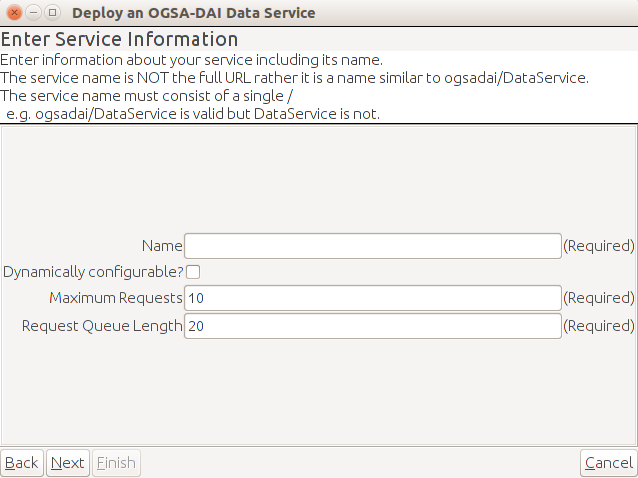
\includegraphics[scale=0.9]{images/guiservice.png}
	\caption{Creazione Data Service tramite GUI}
	\label{guiservice}
\end{figure}


\begin{itemize}
	\item Selezioniamo il percorso relativo al Web Container di Globus e clicchiamo su \textbf{Next}.
	\item Inseriamo l'URL del \textbf{Data Service} o il relative path associato, ad esempio \emph{ogsadai/DataService}.
	\item E' possibile eventualmente specificare il numero di richieste concorrenti che il servizio può supportare e che può accodare quando si raggiunge il limite massimo, attraverso i campi \textbf{Maximum Requests} e \textbf{Request Queue Length}.
\end{itemize}

Per verificare la corretta creazione del servizio sposiamoci nella directory di Globus ed avviamo il Web Container: 

\begin{lstlisting}[language=bash]
$ ./bin/globus-start-container -nosec
\end{lstlisting}

Sarà visualizzata la lista dei servizi disponibili e l'URL al quale è raggiungibile, ad esempio nella forma \emph{http://129.215.56.6:8080/wsrf/services/ogsadai/DataService}. Si noti che una volta creato il servizio è necessario \textbf{riavviare} il Web Container per renderlo disponibile \cite{ogsadai}.

\subsection{Creazione di un Data Service Resource}

In questa sezione descriviamo la procedura per la creazione di una risorsa da esporre presso un servizio, chiamata nel contesto \textbf{Data Service Resource}. Nella Tabella \ref{driverdb} sono presenti i tipi di risorsa supportati da OGSA-DAI ed i relativi driver dei database consigliati per la compilazione \cite{ogsadai}. 


% Please add the following required packages to your document preamble:
% \usepackage[table,xcdraw]{xcolor}
% If you use beamer only pass "xcolor=table" option, i.e. \documentclass[xcolor=table]{beamer}
\begin{table}[H]
	\centering
	\resizebox{\textwidth}{!}{%
		\begin{tabular}{|l|l|l|l|}
			\hline
			\rowcolor[HTML]{C0C0C0} 
			{\bf \begin{tabular}[c]{@{}l@{}}Data\\ Resource\end{tabular}} & {\bf Driver Name} & {\bf JARs} & {\bf Class Name} \\ \hline
			\rowcolor[HTML]{EFEFEF} 
			\multicolumn{4}{|l|}{\cellcolor[HTML]{EFEFEF}{\bf Relazionale}} \\ \hline
			MySQL & MySQL Connector J/2 & \texttt{mysql-connector-java-3.1.8-bin.jar} & org.gjt.mm.mysql.Driver \\ \hline
			DB2 & DB2 JDBC Driver & \begin{tabular}[c]{@{}l@{}}\texttt{db2jcc.jar}\\ \texttt{db2jcc\_licence\_cu.jar}\end{tabular} & \texttt{com.ibm.db2.jcc.DB2Driver} \\ \hline
			SQL Server & Microsoft SQL Server JDBC Driver & \begin{tabular}[c]{@{}l@{}}\texttt{mssqlserver.jar}\\ \texttt{msbase.jar}\\ \texttt{msutil.jar}\end{tabular} & \texttt{com.microsoft.jdbc.sqlserver.SQLServerDriver} \\ \hline
			Oracle & Oracle JDBC Drivers for Java 1.2+ & \begin{tabular}[c]{@{}l@{}}\texttt{classes.zip} \\ rinominato in\\ \texttt{classes.jar}\end{tabular} & \texttt{oracle.jdbc.driver.OracleDriver} \\ \hline
			PostgreSQL & Postgres JDBC Driver & \texttt{pg74.214.jdbc3.jar} & \texttt{org.postgresql.Driver} \\ \hline
			\rowcolor[HTML]{EFEFEF} 
			\multicolumn{4}{|l|}{\cellcolor[HTML]{EFEFEF}{\bf XML}} \\ \hline
			eXist & \texttt{eXist XMLDB Drivers} & \begin{tabular}[c]{@{}l@{}}\texttt{exist.jar}\\ \texttt{xmlrpc-1.2-patched.jar}\end{tabular} & \texttt{org.exist.xmldb.DatabaseImpl} \\ \hline
		\end{tabular}
	}
	\caption{Driver Database Consigliati}
	\label{driverdb}
\end{table}

All'interno della directory di OGSA-DAI WSRF lanciamo il seguente comando: 

\begin{lstlisting}[language=bash]
$ ant guiDeployResource
\end{lstlisting}

\begin{figure}[H]
	\centering
	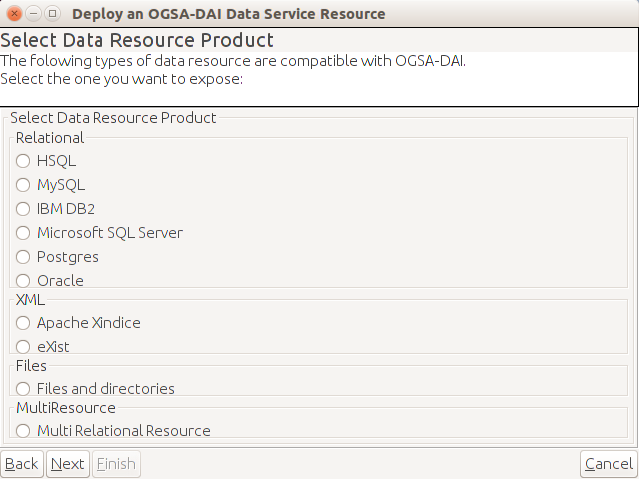
\includegraphics[scale=0.9]{images/guiresource.png}
	\caption{Creazione Data Service Resource tramite GUI}
	\label{guiresource}
\end{figure}

Nella GUI possiamo selezionare tra queste opzioni: 
\begin{itemize}
	\item Creare un Data Service Resource scegliendo tra i vari tipi di risorsa
	\item Caricare un Data Service Resource da un file di configurazione
\end{itemize}
Per le risorse di tipo relazionali ed XML possiamo specificare le seguenti opzioni: 
\begin{itemize}
	\item \textbf{Data Resoruce URI} L'URI della risorsa, compatibile a seconda della classe driver specificata. 
	\item \textbf{Data Resource Driver} Class Driver del database
	\item \textbf{Vendor} Produttore della risorsa (opzionale)
	\item \textbf{Version} Versione della risorsa (opzionale)
	\item \textbf{Vendor} Produttore della risorsa
	\item \textbf{Database access credential} 
	\item \textbf{Database user ID} 
	\item \textbf{Database password} 
	\item \textbf{Data Service Resource ID}
\end{itemize}
Nello step successivo selezioniamo il file JAR relativo al driver del database, ed una volta creata la risorsa clicchiamo su \textbf{Finish} per chiudere la GUI \cite{ogsadai}.

\subsection{Esporre un Data Service Resource}

In questa sezione descriviamo come rendere visibile ed accessibile ai client una risorsa, collegandola ad un servizio attraverso un processo chiamato \emph{Exposing}. 

Nella directory di OGSA-DAI WSRF lanciamo il seguente comando: 

\begin{lstlisting}[language=bash]
$ ant guiExposeResource
\end{lstlisting}

\begin{figure}[H]
	\centering
	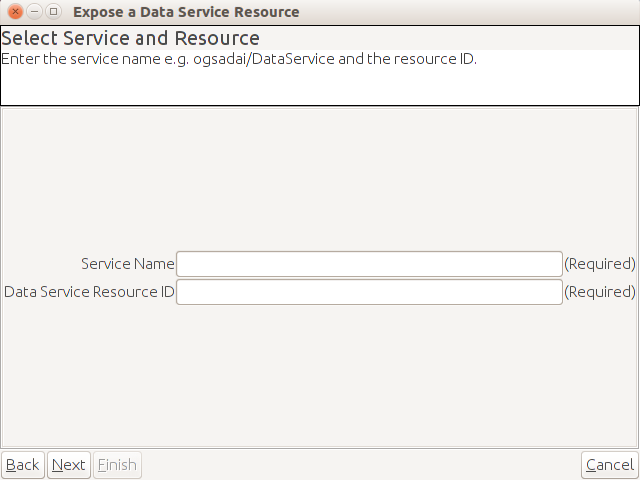
\includegraphics[scale=0.9]{images/guiexpose.png}
	\caption{Expose di un Data Service Resource tramite GUI}
	\label{guiexpose}
\end{figure}

Nella GUI verrà richiesto di inserire le seguenti informazioni: 

\begin{itemize}
	\item Il nome del Data Service, ad esempio \emph{ogsadai/DataService}, nel campo \textbf{Service Name}.
	\item L'ID del Data Service Resource, ad esempio \emph{MyRelationalResource} nel campo \textbf{Data Service Resource ID}.
\end{itemize}

Completata la procedura è necessario riavviare il Web Container per rendere accessibile la risorsa. Possiamo inoltre verificare la corretta associazione del \textbf{servizio/risorsa}, lanciando questo comando sempre nella directory di OGSA-DAI:

\begin{lstlisting}[language=bash]
$ ant listResourcesClient
\end{lstlisting}

Nella shell verrà visualizzata la lista delle risorse attive ed i loro ID, ad esempio: 
\begin{lstlisting}[language=bash]
[java] Service version: OGSA-DAI WSRF 2.2
[java] Number of resources: 2
[java] Resource: MySQLResource
[java] Resource: AnotherResource

\end{lstlisting}

\subsection{End-to-End Client}

Attraverso il cliente End-to-End è possibile: 

\begin{itemize}
	\item Inviare una richiesta ad un servizio per conoscere le risorse che espone
	\item Fare un submit di un \textbf{Perform Document} e ricevere i risultati 
\end{itemize}

Per inviare un Perform Document, e quindi eseguire le Activity definite sulla risorsa (ad esempio una query al database) è necessario che il Web Container sia attivo \cite{ogsadai}. 
Nella directory di OGSA-DAI WSRF lanciamo il seguente comando: 

\begin{lstlisting}[language=bash]
$ ant dataServiceClient -Ddai.url=SERVICE-URL
-Ddai.resource.id=RESOURCE-ID
-Ddai.action=PERFORM-DOC-LOCATION
\end{lstlisting}

Descriviamo ora brevemente i parametri: 

\begin{itemize}
	\item \textbf{dai.url=} Specifica l'URL del Data Service. Se omesso assume come valore di default \emph{http://localhost:8080/wsrf/services/ogsadai/DataService}.
	\item \textbf{dai.resource.id=} Specifica il Data Service Resource al quale il Perform Document sarà sottoposto. 
	\item \textbf{dai.action}= Percorso del Perform Document \cite{ogsadai}.
\end{itemize}

Se le Activity relative al documento vengono eseguite correttamente, la risposta visibile nella shell sarà del seguente tipo: 
\begin{lstlisting}[language=bash]
[echo] Executing Perform document on resource One...
[java] Contacting ... http://localhost:8080/wsrf/services/ogsadai/MyDataService
[java] Service version: OGSA-DAI WSRF 2.2
[java] Number of resources: 2
[java] Resource: MySQLResource
[java] Resource: AnotherResource
[java] Data Service Resource: MySQLResource
[java] About to invoke Perform...
[java] Perform completed!
[java] Response: 
[java] <?xml version="1.0" encoding="UTF-8"?>
[java] <ns1:response xmlns:ns1="http://ogsadai.org.uk/namespaces/2005/10/types">
[java] <request status="COMPLETED"
xmlns="http://ogsadai.org.uk/namespaces/2005/10/service/types"/>

\end{lstlisting}

\subsection{Databrowser}

In OGSA-DAI WSRF è presente un'interfaccia chiamata Databrowser, attraverso cui è possibile gestire tutti le funzionalità descritte in precedenza, dalla creazione di servizi e risorse, esecuzione di Activity etc. Per avviarla, da terminale lanciamo il comando: 

\begin{lstlisting}[language=bash]
$ ant databrowser
\end{lstlisting}

\begin{figure}[H]
	\centering
	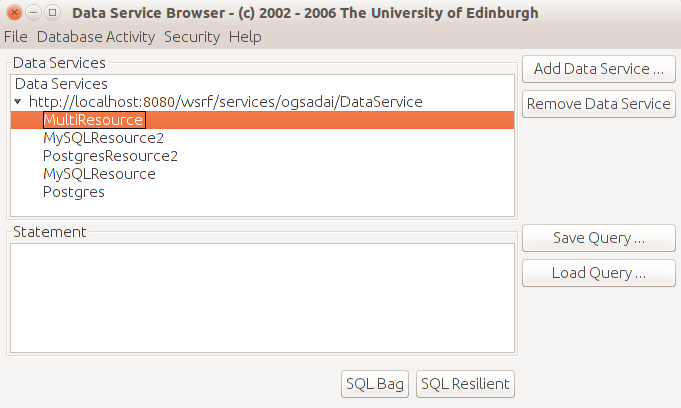
\includegraphics[scale=0.9]{images/databrowser.png}
	\caption{Databrowser GUI}
	\label{databrowser}
\end{figure}

Selezionando una MultiResource è possibile effettuare, su più database, una tipologia di query a seconda del risultato desiderato. Cliccando su \textbf{SQL Bag} verrà effettuato il merge dei risultati, derivanti dall'esecuzione della medesima query su tutte le risorse che il servizio espone. In alternativa, è possibile selezionare \textbf{SQL Resilient} se si desidera sottoporre la query alla prima risorsa esposta disponibile \cite{ogsadai}.
\newpage

\subsection{Creazione di una Multiple Resource}

In questa sezione viene mostrata la procedura per la creazione di una Multiple Resource, al fine di effettuare la query su database multipli. In precedenza sono state create 2 istanze di DBMS collegate alle rispettive risorse, ovvero MySQL Resource e PostegresResource. \\

Presentiamo la struttura dei database usati (\textit{matricola, nomeing,cognomeing,tipoing,universita}), con un riferimento ai dati presenti nel database MySQL. \\

\begin{lstlisting}[language=bash]
15457;"Gianluca";"Abete";"gestionale";"Politecnico di Torino"

32688;"Davide";"Glionna";"elettrico";"Politecnico di Milano"

45879;"Vito";"Fortunato";"informatico";"Politecnico di Bari"

87512;"Giuseppe";"Fiorella";"automatico";"Politecnico di Bari"

95035;"Antonio";"Mastrapasqua";"ambientale";"Politecnico di Torino"

98798;"Carmine";"Del Mastro";"elettronico";"Politecnico di Milano"
\end{lstlisting}

I file di configurazione relativi alle due istanze dei database sono descritti di seguito: 

\begin{lstlisting}[language=bash]

#Database MySQL

dai.resource.id=MySQLResource
dai.data.resource.type=Relational
dai.product.name=MySQL
dai.product.vendor=MySQL
dai.product.version=4.0
dai.data.resource.uri=jdbc:mysql://sql2.freemysqlhosting.net:3306/sql290413
dai.driver.class=org.gjt.mm.mysql.Driver
dai.credential=
dai.user.name=sql290413
dai.password=pF5%qD1%
dai.driver.jars=/home/lordgroove/ogsadai-wsrf-2.2/drivers/mysql-connector-java-5.1.36-bin.jar,
dai.driver.jars.0=/home/lordgroove/ogsadai-wsrf-2.2/drivers/mysql-connector-java-5.1.36-bin.jar
dai.data.service.resource.uri.one=
dai.data.service.resource.id.one=
dai.data.service.resource.description.one=
dai.data.service.resource.uri.two=
dai.data.service.resource.id.two=
dai.data.service.resource.description.two=

\end{lstlisting}

\begin{lstlisting}[language=bash]

#Database Postegres SQL

dai.resource.id=PostgresResource
dai.data.resource.type=Relational
dai.product.name=Postgres
dai.product.vendor=Postgres
dai.product.version=
dai.data.resource.uri=jdbc:postgresql://localhost:5432/postgres
dai.driver.class=org.postgresql.Driver
dai.credential=
dai.user.name=postgres
dai.password=toor
dai.driver.jars=/home/lordgroove/ogsadai-wsrf-2.2/drivers/pg74.214.jdbc3.jar,
dai.driver.jars.0=/home/lordgroove/ogsadai-wsrf-2.2/drivers/pg74.214.jdbc3.jar
dai.data.service.resource.uri.one=
dai.data.service.resource.id.one=
dai.data.service.resource.description.one=
dai.data.service.resource.uri.two=
dai.data.service.resource.id.two=
dai.data.service.resource.description.two=
\end{lstlisting}

Nella root di OGSA-DAI WSRF inseriamo il file di configurazione chiamato \textbf{multi\_config} con le seguenti direttive: 

\begin{lstlisting}[language=bash]
dai.resource.id=MultiResource
dai.data.resource.type=MultiResource
dai.product.name=Multi Relational Resource
dai.data.service.resource.uri.one=http://localhost:8080/wsrf/services/ogsadai/DataService
dai.data.service.resource.id.one=MySQLResource
dai.data.service.resource.uri.two=http://localhost:8080/wsrf/services/ogsadai/DataService2
dai.data.service.resource.id.two=PostgresResource
\end{lstlisting}

Nella subdirectory di Globus \path{/ws-core-4.0.2/etc/ogsadai_wsrf/MultiResource} creiamo un file XML chiamato \textbf{dataResourceConfig.xml} per la creazione del servizio associato alla multi risorsa. 

\begin{lstlisting}[language=xml]
<?xml version="1.0" encoding="UTF-8"?>

<multipleDataResourceConfig
xmlns="http://ogsadai.org.uk/namespaces/2005/10/config" 
xmlns:xsi="http://www.w3.org/2001/XMLSchema-instance"
xsi:schemaLocation="http://ogsadai.org.uk/namespaces/2005/10/config
file:///home/lordgroove/ws-core-4.0.2/share/schema/ogsadai/xsd/multiple_data_resource_config.xsd">

<unitDataServiceConfig>
<dataServiceURL>http://localhost:8080/wsrf/services/ogsadai/DataService</dataServiceURL>
<dataResourceName>MySQLResource</dataResourceName>
<defaultTimeOut>120000</defaultTimeOut>
<maximumTimeOut>600000</maximumTimeOut>
<dataResourceDescription></dataResourceDescription>
<globalSchema></globalSchema>
</unitDataServiceConfig>

<unitDataServiceConfig>
<dataServiceURL>http://localhost:8080/wsrf/services/ogsadai/DataService2</dataServiceURL>
<dataResourceName>PostgresResource</dataResourceName>
<defaultTimeOut>120000</defaultTimeOut>
<maximumTimeOut>600000</maximumTimeOut>
<dataResourceDescription></dataResourceDescription>
<globalSchema></globalSchema>
</unitDataServiceConfig>

</multipleDataResourceConfig>

\end{lstlisting}

Successivamente è stato costruito uno \textbf{script in Java} per testare il funzionamento del servizio creato:

\begin{lstlisting}[language=java]
package uk.org.ogsadai.examples.clienttoolkit;
import uk.org.ogsadai.client.toolkit.GenericServiceFetcher;
import uk.org.ogsadai.client.toolkit.Response;
import uk.org.ogsadai.client.toolkit.activity.ActivityRequest;
import uk.org.ogsadai.client.toolkit.activity.sql.SQLQuery;
import uk.org.ogsadai.client.toolkit.activity.sql.WebRowSet;
import uk.org.ogsadai.client.toolkit.service.DataService;

/**
* Questo esempio crea un Grid Data Service, ed elabora una query SQL. I risultati sono disponibili all'interno di un Perform Document.
*/

public class SimpleSQLQueryExample {
	
	public static void main(String[] args) throws Exception {
		
		// Configurazione servizio URL e ID della risorsa
		String handle = "http://localhost:8080/wsrf/services/ogsadai/DataService";
		String id = "MultiResource";

		if (args.length == 1) {
			handle = args[0];
		}
		
		// Trova il Data Service
		DataService service = GenericServiceFetcher.getInstance().getDataService(handle, id);
		System.out.println("Connessione al data service " + service.getURL());
		
		// Esecuzione QUERY
		String sql = "select * from ingegneri where nome='Giacomo'";
		System.out.println("\nEsecuzione Query: " + sql);
		SQLQuery query = new SQLQuery(sql);
		WebRowSet rowset = new WebRowSet(query.getOutput());
		ActivityRequest request = new ActivityRequest();
		request.add(query);
		request.add(rowset);
		Response response = service.perform( request );
		System.out.println("Risultato:\n" + response.getAsString());	
	}
}
\end{lstlisting}

\newpage

\subsection{Questionario di Autovalutazione}
\textbf{Descrivere brevemente l'architettura WSRF (Web Service Resource Framework)}\\[5ex]
\rule[5mm]{\textwidth}{0.1mm} 
\rule[5mm]{\textwidth}{0.1mm} 
\rule[5mm]{\textwidth}{0.1mm} 
\rule[5mm]{\textwidth}{0.1mm} 
\textbf{Descrivere brevemente un Perform Document e fornire un esempio di una sessione SQL}\\[5ex]
\rule[5mm]{\textwidth}{0.1mm} 
\rule[5mm]{\textwidth}{0.1mm} \\\\\\\\\\\\\\\\\\\\\\\\\\\\\\\\\\\\\
\textbf{Scrivere quali sono i prerequisiti necessari per l'installazione di OGSA-DAI WSRF}\\[5ex]
\rule[5mm]{\textwidth}{0.1mm} 
\rule[5mm]{\textwidth}{0.1mm} 
\rule[5mm]{\textwidth}{0.1mm} 
\textbf{Indicare attraverso quali dei seguenti toolkit di OGSA-DAI WSRF è possibile effettuare un submit di un Perform Document (indicare una o più risposte): }
\begin{enumerate}
	\voceU{End-to-end Client}
	\voceU{Expose Resource}
	\voceU{Databrowser}\\
\end{enumerate}
\newpage


\section{Implementazione dei Big Data nel Grid Computing}
\textbf{Big Data} è un termine che definisce il concetto di dati, aventi 3 \emph{caratteristiche} fondamentali. 
\begin{enumerate}
	\item Grande quantità di dati
	\item Dati non strutturati in tabelle come nei DB relazionali
	\item Dati generati, recuperati ed elaborati con estrema velocità
\end{enumerate}

\emph{Oracle} inoltre, ha aggiunto una quarta caratteristica per questa tipologia di dati, ovvero una \textbf{bassa densità di informazione esplicita}, la quale implica che alcune volte, prima di cercare le informazioni necessarie, bisogna processare una grande quantità di dati. Big Data è relativamente un nuovo termine che nasce dalle necessità delle big companies come \emph{Yahoo}, \emph{Google}, \emph{Facebook} al fine di analizzare ingenti quantità di dati non strutturati. Tuttavia la tematica è di notevole interesse anche per altre imprese che investono nel campo Ricerca e Sviluppo \cite{6511732}. 

Il \emph{framework} per elaborare i Big Data che sarà in seguito analizzato, prende il nome di \textbf{Hadoop} \cite{hadoop}.
Hadoop è costituto dai seguenti componenti: 
\begin{enumerate}
	\item Hadoop kernel
	\item Hadoop Distributed File System (HDFS)
	\item MapReduce
	\item Ulteriori componenti aggiuntivi
\end{enumerate}
I problemi principali che si incontrano quando si affronta la tematica sui Big Data, consistono nella capacità di memorizzazione, e della potenzialità di calcolo. Infatti, la tecnologia risolutiva che consente di risolvere tali problematiche, è fornita dalle \emph{griglie computazionali}. Consideriamo una griglia come un sistema definito da un \textbf{Computing Element} (CE), \textbf{Storage Element} (SE) e \textbf{Worker Node} (WN) \cite{6511732}. 

Il CE fornisce il servizio di connessione con altre reti GRID ed utilizza un \emph{Workload Management System} per gestire ed trasmettere i job sui Worker Node. Lo Storage Element si occupa della memorizzazione dei dati di input e di output, necessari all'esecuzione del job. Mentre i Worker Node sono solitamente server che forniscono la necessaria potenzialità di calcolo \cite{6511732}.

\subsection{Cosa sono attualmente i Big Data}
Oggigiorno, viviamo in un contesto interconnesso che genera un grande volume di informazioni, a partire dai file di log degli utenti presenti sui social network, motori di ricerca, dati di monitoraggio provenienti dalle \textbf{Wireless Sensor Networks} (WSN), e-mail fino ad arrivare alle reti veicolari, centri di ricerca e così via. Da un'infografica prodotta da Intel, si nota come oggi il 90\% dei dati è stato creato negli ultimi due anni, ed è in costante crescita. Si stima infatti che tutti i dati a livello globale, generati fino al 2003 rappresentano circa 5 exaByte (1 exaByte è pari a 1 milione di gigaByte); l'ammontare dei dati generati fino all'anno 2012 invece è pari a 2.7 zettaByte (1 zettaByte è pari a 1000 exaBytes). Si prospetta quindi che al termine dell'anno 2015, questo valore venga triplicato.Ad esempio, il numero dei dispositivi RFID venduti nell'anno 2012 era pari a circa 12 milioni, mentre oggi si è stimato che questo numero diventi pari a 209 bilioni nel 2021 \cite{6511732}.

Quando si parla di Big Data, ci si riferisce subito a grandi quantità di dati, ma in realtà il concetto va ben oltre questo aspetto. I dati come sappiamo, vengono presentati in modo eterogeneo, tipo strutturati, semi-strutturati, non strutturati. Inoltre anche il modo con cui viene processato il dato varia, difatti tutto dipende dall'analisi che deve essere fatta in seguito o dall'informazione che si desidererà cercare all'interno dei dati iniziali \cite{6511732}. 

Di solito, queste grandi quantità di dati sono prodotte con elevate velocità, richiedendo tempi di elaborazioni piuttosto rapidi, come accade nel caso di monitoraggio di uno scenario, effettuato in tempo reale \cite{6511732}.

\subsection{Come processare i Big Data}
Questa tipologia di dati, è impossibile da gestire utilizzando i tradizionali DBMS relazionali. Le nuove tecnologie innovative, sono state messe a punto da \emph{Google}, sfruttando un modello denominato \textbf{MapReduce}. In realtà, sono molteplici le soluzioni per poter gestire i Big Data, ma quella maggiormente usata è Hadoop \cite{6511732} \cite{hadoop}.

Hadoop è un framework \textbf{open source} basato sul modello MapReduce di \emph{Google} e sul \emph{Google File System}. Hadoop è stato fondato dall'\textbf{Apache Software Foundation}. I suoi collaboratori al progetto sono \emph{Yahoo}, \emph{Facebook}, \emph{Citrix}, \emph{Google}, \emph{Microsoft}, \emph{IBM}, \emph{HP}, \emph{Cloudera} e tanti altri. Il framework che consente lo sviluppo di applicazioni distribuite con numerosi accessi ai dati, è costituito dai seguenti componenti principali:
\begin{enumerate}
	\item Hadoop Kernel
	\item Hadoop Distributed File System (HDFS)
	\item MapReduce
	\item Componenti per il Data Access, Management come in Figura \ref{archdopp}
\end{enumerate}

\begin{figure}[H]
	\centering
	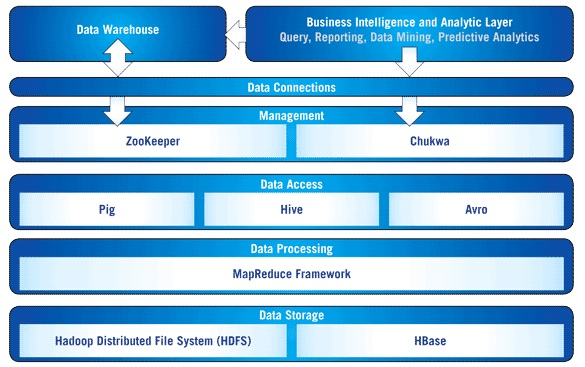
\includegraphics[scale=0.93]{images/hadoop-architecture.jpg}
	\caption{Architettura di Hadoop \cite{hadoop}}
	\label{archdopp}
\end{figure}

\begin{enumerate}
	\item [A.]\emph{HDFS}
	
	\textbf{HDFS} è un file system strutturato a blocchi distribuito, progettato per gestire grandi quantità di dati in modo affidabile, scalabile in maniera semplice. I blocchi vengono chiamati chunk, definiti da una dimensione predefinita di 64 MB (eccetto per l'ultimo blocco di ogni file), molto più grande dell'usuale 4 o 8 KB nella maggior parte del file system strutturati a blocchi. HDFS ha un'architettura client-server costituita da un \textbf{NameNode} e molti \textbf{DataNode} \cite{hadoop}.
	
	Il \emph{NameNode} ha il compito di memorizzare i metadati per i \emph{DataNode}. I metadati sono definiti da un nome, permessi, fattore di replica e locazione del chunk sul DataNode. Esso consente di salvarli in memoria, così da poter garantire un incremento della velocità di accesso ai dati, in termini di operazioni al secondo. Il NameNode è responsabile anche delle operazioni sul file system, come l'apertura, la chiusura, lo spostamento, e rinomina di file e cartelle. Inoltre, esso tiene traccia dello stato dei DataNode, mediante la ricezione di segnali chiamati heartbeats \cite{hadoop}.
	
	\item [B.]\emph{I vantaggi principali offerti da Hadoop}
	
	HDFS offre un'elevata portabilità, dal momento che è stato scritto in Java e progettato per essere compatibile sulla maggior parte dell'hardware presente in circolazione. Di solito viene eseguito su elaboratori dotati di sistema operativo GNU/Linux. HDFS offre una grande affidabilità grazie al fatto che tutti i file vengono replicati su due o più DataNode. Il numero predefinito di repliche è pari a tre. La dimensione del blocco e il fattore di replica, sono configurabili per ogni singolo file. Lo schema per la replica, viene gestito dal NameNode ed eseguito dal DataNode in base alle istruzioni provenienti dal NameNode. Sfortunatamente, Hadoop non supporta l'\emph{automatic recovery} nel caso in cui un NameNode dovesse danneggiarsi \cite{hadoop}. 
	
	Ciò che si potrebbe fare, è definire un \textbf{SecondaryNameNode} da configurare su un'altra macchina. Quest'ultimo non sarà il sostituto del NameNode in caso di guasto; ciò significa che i DataNode non potranno collegarsi ad esso, ma che periodicamente effettueranno dei checkpoint: esso effettuerà il download dell'immagine della macchina NameNode modificando di conseguenza anche i file di log; successivamente verrà creata una nuova immagine che potrà essere caricata sul NameNode primario. Al fine di poter prevenire errori di sincronizzazione tra l'informazione contenuta nel NameNode e ciò che è realmente presente sui DataNode, HDFS richiederà un report per ogni blocco dai DataNode \cite{hadoop}.
	
	Tuttavia, l'integrità dei dati sui DataNode, è verificata mediante un checksum su ogni rispettivo blocco. Nel caso in cui, il checksum dovesse fallire, i blocchi danneggiati saranno eliminati e sostituiti dal NameNode.
	HDFS è basato sul principio "\textbf{Moving Computation is Cheaper than Moving Data}" (MCCMD), il che significa che è più semplice spostare la computazione sui dati ancora da elaborare, invece che spostare i dati dove la computazione è stata già avviata. Questo concetto risulta particolarmente utile, quando le operazioni di I/O avvengono su file di notevoli dimensioni \cite{hadoop}.
\end{enumerate} 

\subsection{Implementare una piattaforma per i Big Data in un Grid Center}
Hadoop è stato scritto principalmente per il trasferimento dei dati effettuato su uno stesso data center, nonostante sia stato sviluppato per la distribuzione dei dati su griglie computazionali.
Lo scheduler di Hadoop tenta di collocare al buon 70\% o più i suoi job ed i suoi dati, così da garantire la presenza dei dati di input su dischi locali dei \emph{Working Node} della griglia.
\emph{Come si potrebbe usare Hadoop in una griglia computazionale ?} \cite{hadoop}

Ci sono state molteplici implementazioni all'interno dei Grid Center. Ad esempio, analizziamo l'architettura definita da uno Storage Element che utilizza il framework Hadoop. Esso è composto da DataNode dedicati, sui quali è presente Hadoop Client, ma anche da DataNode che sfruttano le capacità di storage dei rispettivi WN presenti nel Grid Center. Naturalmente, è necessaria la presenza di un altro server che gestisca il job del NameNode e tenga traccia della relativa locazione dei dati.
Poichè HDFS non implementa tutte le interfacce POSIX, il supporto viene fornito da \textbf{FUSE} \cite{fuse}. 

\emph{Fuse} (Filesystem in Userspace) è un modulo del kernel del sistema operativo Unix, che consente di effettuare il mount di un file system all'interno di uno userspace. FUSE consente quindi di effettuare il mounting relativo al file system del SE, e di essere visto da parte del WN come un file system locale, offrendo una interfaccia simile alla POSIX \cite{fuse}.
Nei primi mesi del 2012, Oracle ha stretto un accordo con Cloudera per portare Apache Hadoop in \emph{Oracle Big Data Appliance}. I dispositivi sono dotati della distribuzione Cloudera con Apache Hadoop incluso (\textbf{CDH}), in aggiunta con il software Cloudera Manager. Questa architettura è stata utilizzata per applicazioni relative all'analisi di Big Data \cite{fuse}.

\begin{figure}[H]
	\centering
	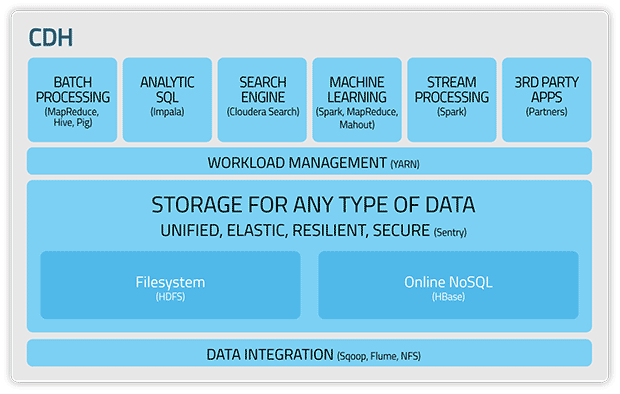
\includegraphics[scale=0.65]{images/CDH_diagram.png}
	\caption{Diagramma dell'architettura CDH \cite{6511732}}
	\label{cdh}
\end{figure}

\subsection{Conclusioni}
I vantaggi principali offerti dal Grid Computing sono le capacità di storage, la potenzialità di calcolo ed i benefici principali derivanti dall'uso di Hadoop:
\begin{enumerate}
	\item HDFS
	\item Affidabilità (offerta sia dalla replica di tutti i dati presenti sui DataNode e sia dagli altri nodi configurati in caso di malfunzionamento)
	\item Capacità dello scheduler nel collocare i job ed i dati, garantendo quindi un elevato \emph{throughput} dal job
	\item Semplicità di utilizzo
	\item Manutenzione
	\item Scalabilità
\end{enumerate}

L'approccio di \emph{Oracle/Cloudera} oltre ad essere interessante, è un'ottima combinazione degli strumenti software messi a disposizione da Cloudera, e dai sistemi ingegneristici proposti da Oracle, in grado di fornire elevate performance e scalabilità nell'elaborazione dei Big Data.


\newpage

\subsection{Questionario di Autovalutazione}
\textbf{Quali sono le tre caratteristiche fondamentali  dei Big Data ? Enunciare inoltre, se esiste e spiegare in cosa consisterebbe la quarta caratteristica.}\\[5ex]
\rule[5mm]{\textwidth}{0.1mm} 
\rule[5mm]{\textwidth}{0.1mm} 
\rule[5mm]{\textwidth}{0.1mm} 
\rule[5mm]{\textwidth}{0.1mm} 
\rule[5mm]{\textwidth}{0.1mm} 
\rule[5mm]{\textwidth}{0.1mm} 
\textbf{Descrivere il funzionamento del framework MapReduce.}\\[5ex]
\rule[5mm]{\textwidth}{0.1mm} 
\rule[5mm]{\textwidth}{0.1mm} 
\rule[5mm]{\textwidth}{0.1mm} 
\rule[5mm]{\textwidth}{0.1mm} 
\rule[5mm]{\textwidth}{0.1mm} 
\rule[5mm]{\textwidth}{0.1mm} 
\textbf{Quali sono i vantaggi offerti dall'uso di Hadoop ?}
\begin{enumerate}
	\voceU{HDFS, affidabilità, manutenzione}
	\voceU{Scalabilità, semplicità di utilizzo}
	\voceU{Portabilità, sicurezza, trasparenza}
	\voceU{Manutenzione, NTFS, scalabilità}\\
\end{enumerate}
\textbf{Disegnare e descrivere il Diagramma dell'architettura CDH.}\\\\\\\\\\\\\\\\\\\\\\\\\\\\\\\\\\
\newpage


\section {Introduzione all'Hybrid Data Infrastructure}
Una \emph{Hybrid Data Infrastructure} (HDI) è una nuova tipologia di infrastruttura dati concepita per l'elaborazione di ingenti quantità di dati scientifici. In tale dominio, i dataset vengono distribuiti sia dal singolo laboratorio di ricerca e sia dai molteplici centri di ricerca e sviluppo. La gestione e l'elaborazione richiesta da tali dataset, va al di là delle capacità relative alle tecnologie tradizionali. Tali dati sono caratterizzati dalle 3 V:
\begin{enumerate}
	\item \emph{Volume} (\textbf{Volume}): Grandi dimensioni dei dati in termini di byte.
	\item \emph{Velocity} (\textbf{Velocità}): Velocità di elaborazione e trasmissione dei dati.
	\item \emph{Variety} (\textbf{Eterogeneità}): Elevata integrazione dei dati da sorgenti differenti \cite{candela2012managing}.
\end{enumerate}

Una \textbf{Hybrid Data Infrastructure} è una tecnologia innovativa basata sull'assunzione che diverse architetture fisiche di sistemi distribuiti per il calcolo e lo storage, tra cui le \textbf{griglie computazionali}, il \textbf{Cloud Computing}, e così via, possono essere integrate per fornire sia un accesso efficiente che un uso/gestione dei dati attendibile \cite{candela2012managing}.
Recenti studi, infatti, evidenziano come tali tecnologie, utilizzate per molti anni in maniera indipendente, presentino difficoltà nella gestione di dataset eterogenei. Da una parte, il Grid Computing presenta soluzioni per \textbf{problemi di "varietà" dei dati}, attraverso complesse implementazioni di middleware ed ingenti risorse hardware, spesso regolate da politiche e procedure rigide \cite{candela2012managing}.

Dall'altra, il Cloud Computing è un paradigma di utilizzo di risorse di calcolo, basato sulla gestione delle risorse in maniera elastica, affidando i costi di manutenzione dell'hardware, middleware e dell'infrastruttura (centralizzati) a produttori di terze parti. L'uso del Cloud Computing viene rilasciato in termini di servizi(IaaS, SaaS, PaaS) all'utente finale, con un abbattimento dei relativi costi. Tuttavia, l'interazione diretta tra producer e consumer impedisce, in molti casi, l'integrazione nel Cloud di risorse sviluppate da organizzazioni dislocate geograficamente in maniera sparsa \cite{candela2012managing}.

L'architettura, deve essere dotata di diversi servizi di mediazione, che consentano di interfacciarsi con basi di dati esistenti. Nel complesso, l'obiettivo è quello di fornire un modello per la gestione dei dati, nel quale, la capacità di calcolo, la memorizzazione dei dati, il software e le informazioni siano disponibili grazie all'uso di questa \textbf{IaaS} (\emph{Infrastructure as a Service}) \cite{candela2012managing}.

\subsection{gCube Framework}

gCube è un framework sviluppato in collaborazione con ISTI-CNR, propone un nuovo scenario di infrastruttura dati distribuita, secondo l'approccio HDI. E' stato inizialmente concepito per amministrare architetture per il calcolo distribuito classiche, per poi evolversi secondo il modello HDI su larga scala, creando un sistema unico per l'accesso, lo storage ed il computing, attraverso un client Web molto leggero con la creazione di \textbf{Virtual Research Environments} dedicati \cite{candela2012managing} \cite{candela2008gcube}. 

gCube è in grado di interagire con una vasta gamma di risorse computazionali e di storage, attraverso una serie di\textbf{ Mediator Services} che permettono l'interfacciamento con le Grid (ad esempio European Grid Infrastracture), servizi cloud commerciali (Microsoft Azure, Amazon EC2), e Private Cloud(OpenNebula), database relazionali e sistemi di storage geospaziali (Geoserver), database NoSQL (Cassandra, MongoDB), e piattaforme di computing distribuite (Hadoop) \cite{candela2012managing} \cite{candela2008gcube}.

\begin{figure}[H]
	\centering
	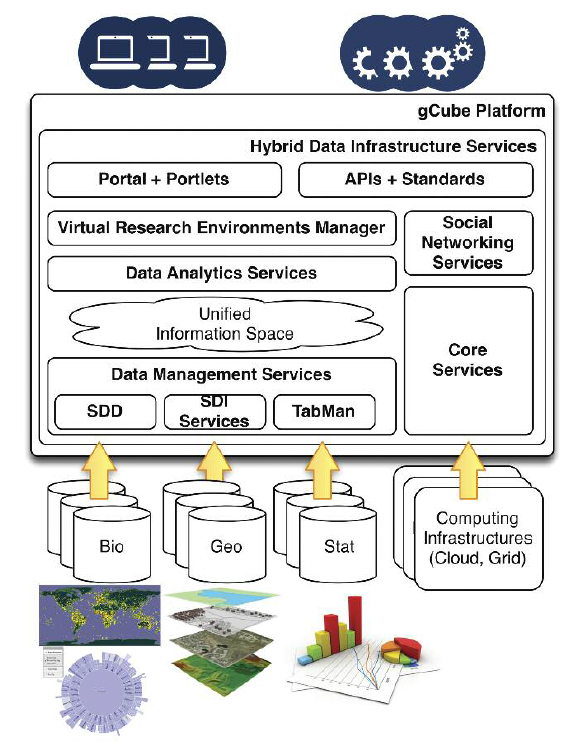
\includegraphics[scale=0.6]{images/gcube.png}
	\caption{Architettura di gCube \cite{candela2012managing}}
	\label{gcube}
\end{figure}

\subsection{BIGhybrid - Un Toolkit per simulare MapReduce su Hybrid Data Infrastructure}
Coniugando il cloud computing con le griglie computazionali, si ottiene una soluzione flessibile e a basso costo per l'analisi dei big data. I framework come \emph{MapReduce} sono stati messi a punto al fine di sfruttare l'hardware a disposizione, affrontando di conseguenza mediante le hybrid infrastructure le sfide inerenti all'integrazione delle risorse eterogenee. Sono stati presentati diversi tool, tra cui vale la pena citare \textbf{BIGhybrid}, un toolkit per simulare MapReduce su ambienti ibridi \cite{6972028}. 

BIGhybrid è in grado di simulare due architetture middleware per due differenti tipologie di infrastrutture: BitDew-MR, per griglie computazionali e Hadoop-Blobseer per il Cloud computing. BIGhybrid possiede varie caratteristiche: implementato e basato su MRSG (MapReduce over SimGrid), un simulatore Hadoop, ed MRA++(MapReduce Adapted Algorithms to Heterogeneous Environments), un simulatore per ambienti eterogenei; il tool possiede un trace toolkit che è in grado di analizzare, monitorare e mostrare graficamente i task in esecuzione \cite{6972028}.

BIGhybrid può essere usato per la valutazione inerente alle strategie di scheduling per applicazioni multirisorsa su infrastrutture ibride \cite{6972028}.

In Figura \ref{bighybridarch} possiamo dare uno sguardo all'architettura di BIGhybrid Simulator. Agli elementi già citati, si aggiungo un \emph{Global Dispatcher} per la gestione dei dati di input, i moduli \emph{Cloud-BlobSeer}, \emph{BitDew-MapReduce} e \emph{Global Aggregator} per l'integrazione dei risultati \cite{6972028}.

\begin{figure}[H]
	\centering
	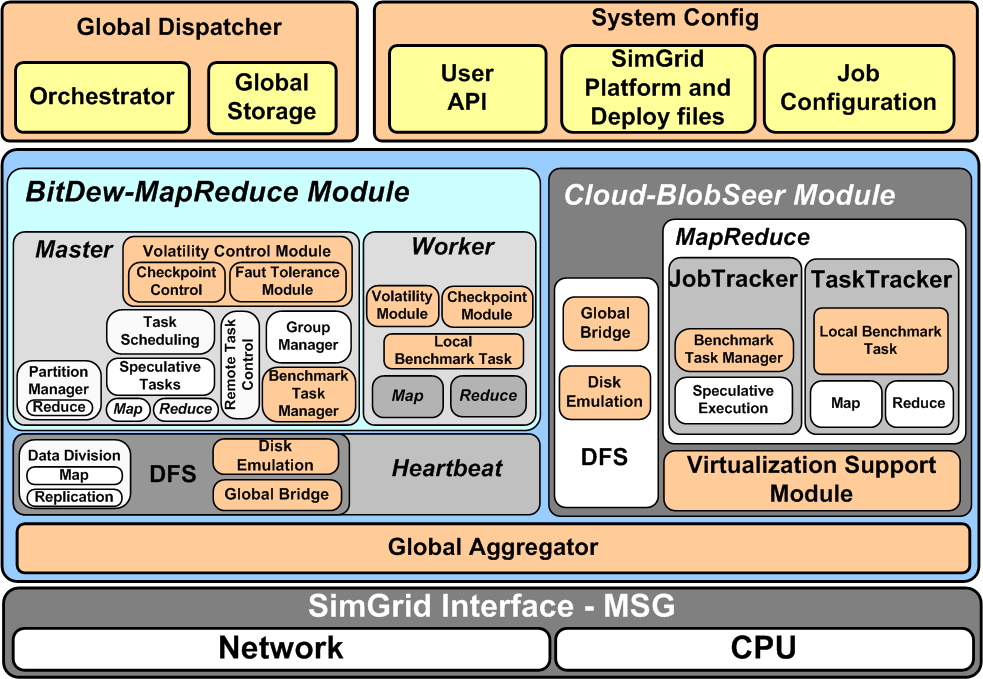
\includegraphics[scale=0.40]{images/bighybridarch.png}
	\caption{Architettura di BIGhybrid Simulator \cite{6972028}.}
	\label{bighybridarch}
\end{figure}

\newpage

\subsection{Questionario di Autovalutazione}
\textbf{Descrivere che cos'è l'Hybrid Data Infrastructure.}\\[5ex]
\rule[5mm]{\textwidth}{0.1mm} 
\rule[5mm]{\textwidth}{0.1mm} 
\rule[5mm]{\textwidth}{0.1mm} 
\rule[5mm]{\textwidth}{0.1mm} 
\textbf{Quali proprietà caratterizzano i dataset che una HDI è in grado di gestire (dette proprietà delle 3 V)? }
\begin{enumerate}
	\voceU{Visibilità, Velocità, Varietà}
	\voceU{Volume, Velocità, Varietà}
	\voceU{Volume, Velocità, Visibilità}\\
\end{enumerate}
\textbf{Cosa si intende per SaaS, PaaS, IaaS ?}\\[5ex]
\rule[5mm]{\textwidth}{0.1mm} 
\rule[5mm]{\textwidth}{0.1mm} 
\rule[5mm]{\textwidth}{0.1mm} 
\rule[5mm]{\textwidth}{0.1mm} 
\textbf{Descrivere il framework gCube ed il toolkit BigHybrid.}\\[5ex]
\rule[5mm]{\textwidth}{0.1mm} 
\rule[5mm]{\textwidth}{0.1mm} 
\rule[5mm]{\textwidth}{0.1mm} 
\rule[5mm]{\textwidth}{0.1mm} 

\newpage


\clearpage
\addcontentsline{toc}{section}{Bibliografia}
\nocite{*}
\bibliographystyle{plain}
\bibliography{biblib}




\end{document}